\subsection{Entwurf}\label{l:entwurf}

Diese vier Leitlinien repräsentieren die Grundgedanken bei der Entwicklung von der Anwendung:

\begin{itemize}
\item{Das wichtigste zuerst: Die aktuelle Aufgabe soll immer im Fokus der Darstellung liegen.}
\item{Schnell zum Ziel: Alle Aufgaben müssen leicht und umkompliziert durchführbar sein.}
\item{Nicht nerven: Ständige Benachrichtigungen lenken ab und müssen deswegen so gestaltet sein, dass diese sich nach den Präferenzen des Nutzers richten.}
\item{Hilfe nur einen Klick entfernt: Das Hilfesystem muss kontextsensitiv verfügbar sein und ist eine Kernfunktion der Anwendung}
\end{itemize}

\subsubsection{Überblick}

Diese Abbildung liefert einen Überblick über den Aufbau des Systems:

\begin{figure}[htb]
\begin{center}
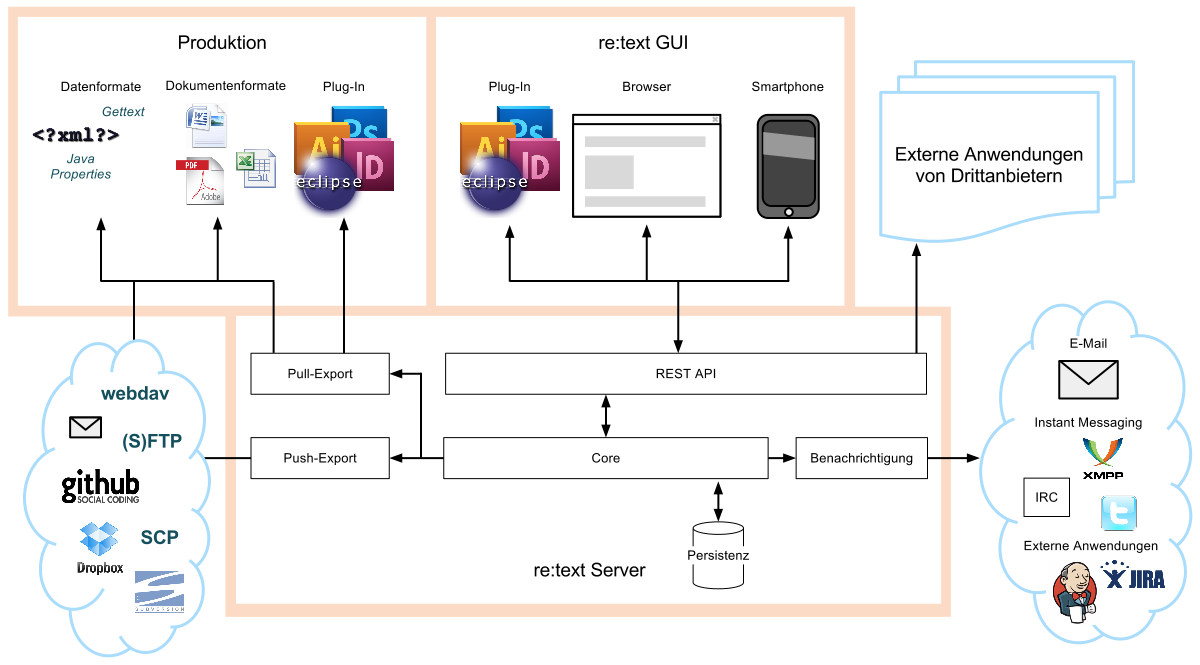
\includegraphics[width=\textwidth]{media/System.pdf}
\caption{Aufbau des Systems}
\label{chart:1}
\end{center}
\end{figure}

Die Zentrale Komponente der Anwendung bildet der Server. Für die Benutzer erfolgt der Zugriff mit Hilfe einer GUI, die mit der REST-API des Servers kommuniziert. In der ersten Version wird eine browserbasierte GUI auf Basis von HTML5 und JavaScript existieren, die auch schon auf Smartphones verwendet werden kann. Später kommen dann spezielle Plugins für Adobe-Produkte und weitere wichtige Produktionsumgebungen hinzu. Auch native GUIs für Smartphones verwenden die gleiche API. Die Schnittstellen können auch von Drittanbietern dazu verwendet werden, eigenen Clients für das System zu entwickeln. In die Endprodukte gelangen die Texten über den Export, exportiert wird dabei in viele Formate, neben Datenformaten wie z.B. XML werden auch Dokumentenformate wie z.B. Word exportiert. Der Export kann durch den Anwender erzeugt werden (\emph{Pull-Export}), aber auch automatisch, z.B. nach festgelegten Zeitplänen oder Ereignissen erfolgen. Dieser \emph{Push-Export} erfolgt auf je nach Projekt festlegbaren Orte, wie z.B. FTP-Server oder Versionsverwaltungssysteme. Die Benachrichtigungen über Aufgaben und Änderungen an Texten kann via E-Mail, aber auch mittels Instant-Messaging-Systeme oder durch den Aufruf fremde API-Endpunkte erfolgen – dies ist ebenfalls innerhalb eines Projektes und pro Nutzer individuell konfigurierbar.

\subsubsection{Grundüberlegung zu einer GUI}

Anforderungen, Grundsätze, Usability, Aufbau, Wireframes

Bei Kontroll-Aufgaben (Lektorat, QS) unterbrechungsfreies Arbeiten ermöglichen (Infinite-Scroll).

Die GUI muss deutlich einfacher zu bedienen sein, als z.B. Word oder Publishing-Systeme, sonst wird sie nicht von Kunden eingesetzt.